\documentclass[a4paper]{article}

\usepackage[utf8]{inputenc}
\usepackage[T1]{fontenc}
\usepackage{textcomp}
\usepackage[czech]{babel}
\usepackage{amsmath, amssymb}


% figure support
\usepackage{import}
\usepackage{xifthen}
\pdfminorversion=7
\usepackage{pdfpages}
\usepackage{transparent}
\newcommand{\incfig}[1]{%
    \def\svgwidth{\columnwidth}
    \import{./figures/}{#1.pdf_tex}
}

\pdfsuppresswarningpagegroup=1
\author{Hynek Kydlicek}
\title{Diskrétka 7}
\begin{document}
\maketitle
\section{Úkol 1}%
Ukážeme, že pokud je velikost jedné z parit $\ge  3$, doplněk takového grafu není bipartitní.
Označme si partity $A,B$. Z definice bipartitního grafu $G$ pro doplněk $G'$ platí $(\forall v_1,v_2 \in A) (\{v_1, v_2\} \in E')$. Tedy žádné 2 vrcholy z A nesmí být ve stejné partitě v novém $G'$. Partity máme jenom 2, proto $|A| \le 2 \wedge |B| \le 2$.
Tedy $2 \le n \le  4$. Ukážeme, že takové grafy a jejich doplňky opravdu existují viz. obr. \ref{fig:bip-graf}.
\begin{figure}[htpb]
    \centering
    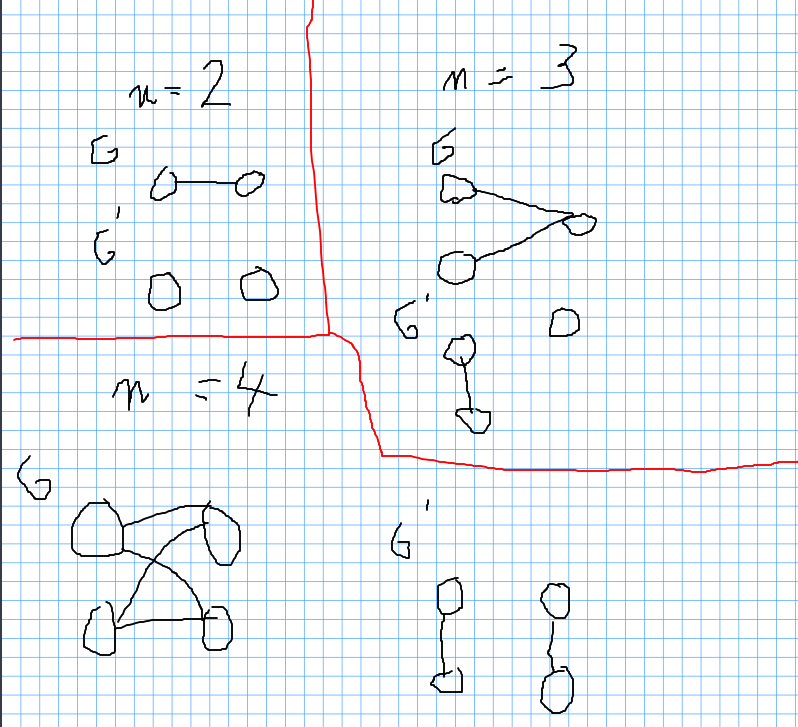
\includegraphics[width=0.5\textwidth]{1.png}
    \caption{Bipartitní graf}
    \label{fig:bip-graf}
\end{figure}

\section{Úkol 2}%
\subsection{Počet úplných bipartitních grafů}
V textu budou všechny bipartitní grafy úplné.
Počet různých úplných bipartitních grafů na n vrcholech s velikostí partit $k, n-k = {n\choose k}$.
Vybíráme k vrcholů z n prvků do první partity, druhá je určena jednoznačně.
Zároveň je nutné si uvědomit, že pokud k = n-k, pak výsledek musíme ještě vydělit 2, protože graf s partitami $A=\{a_1, a_2 \dots a_k\}, B = \{b_1, b_2 \dots b_k\} $ je stejný jako graf s paritami $B=\{a_1, a_2 \dots a_k\}, A = \{b_1, b_2 \dots b_k\} $.

Nyní stačí sečíst počet všech různých bipartitních grafů pro všechna $k \in \{1, n-1\}$.
Uvědomíme si, že množina různých bipartitní grafů k, n-k je stejná jako množina různých bipartitních grafů n-k, n.
Tedy výsledný počet musíme vydělit 2.
Dostáváme, že počet různých úplných bipartitních grafů je.
\begin{align*}
    &\text{Pro sudá n: }
    \sum_{k = 1}^{\frac{n}{2}-1} {n \choose k} + \frac{{n \choose \frac{n}{2}}}{2} = \sum_{k=1}^{n-1} \frac{{n \choose k}}{2}
    \\
    &\text{Pro lichá n:}
    \sum_{k=1}^{n-1} \frac{{n \choose k}}{2}
\end{align*}

\subsection{Počet kružnic délky n}
Počet všech možností jako očíslovat vrcholy $= n!$.
Uvědomíme si, že pokud očíslujeme vrcholy $1, 2, 3 \dots n$ je to stejný graf jako $n, 1, 2, 3 \dots n-1$.
Takových posunů je $n$. Zárověn očíslovaní $1, 2, 3 \dots n$ je stejné jako $1, n, n-1 \dots 3, 2$.
\begin{align*}
    \text{Počet různých kružnic: }
    \frac{n!}{2*n}
.\end{align*}

\section{Úkol 3}
Ukážeme že 7-regulární graf na 15 vrcholech musí být nutně souvislý.
Pro ostatní grafy, kde mají všechny vrcholy stupeň $\ge 7$ to bude triviálně platit taky, přidáním hrany nemůže graf udělat nesouvislý.
\\
Pokud by nebyl 7-regulární graf souvislý, musela by minimální velikost každé komponenty souvislosti být alespoň 8 (z každého vrcholu musí vést hrana do 7 dalších vrcholů, tyto vrcholy jsou nutně souvislé). Tedy počet vrcholů by musel být alespoň 16. To je spor s předpokladem, že vrcholů je 15.

\end{document}
